
Likewise, the objective of chapter 4 is to describe the researcher's design 
consideration when developing and testing the prototype. For an overview of 
the design of the prototype, the researchers considered different computer vision models in
 classifying the ripeness and bruises together with other algorithms to determine 
 the size of the mango. Likewise, the hardware design was also taken into consideration where 
 the physical design of the conveyor belt was taken into account.

\section{Introduction}
This chapter discusses the design considerations for the mango 
sorting and grading system, focusing on the technical and engineering decisions 
required for its development. The design process aims to create a scalable, efficient, 
and user-friendly system that leverages machine learning for accurate mango classification.

\section{System Architecture}
The system architecture is represented through a block diagram, showcasing modules such as image acquisition, 
preprocessing, feature extraction, machine learning model, and grading output. Each module is described in detail, 
emphasizing its role in the overall system. For instance, the image acquisition module uses high-resolution cameras 
to capture mango images, while the preprocessing module enhances image quality for better feature extraction.

\begin{figure}[!htbp]
	\centering
	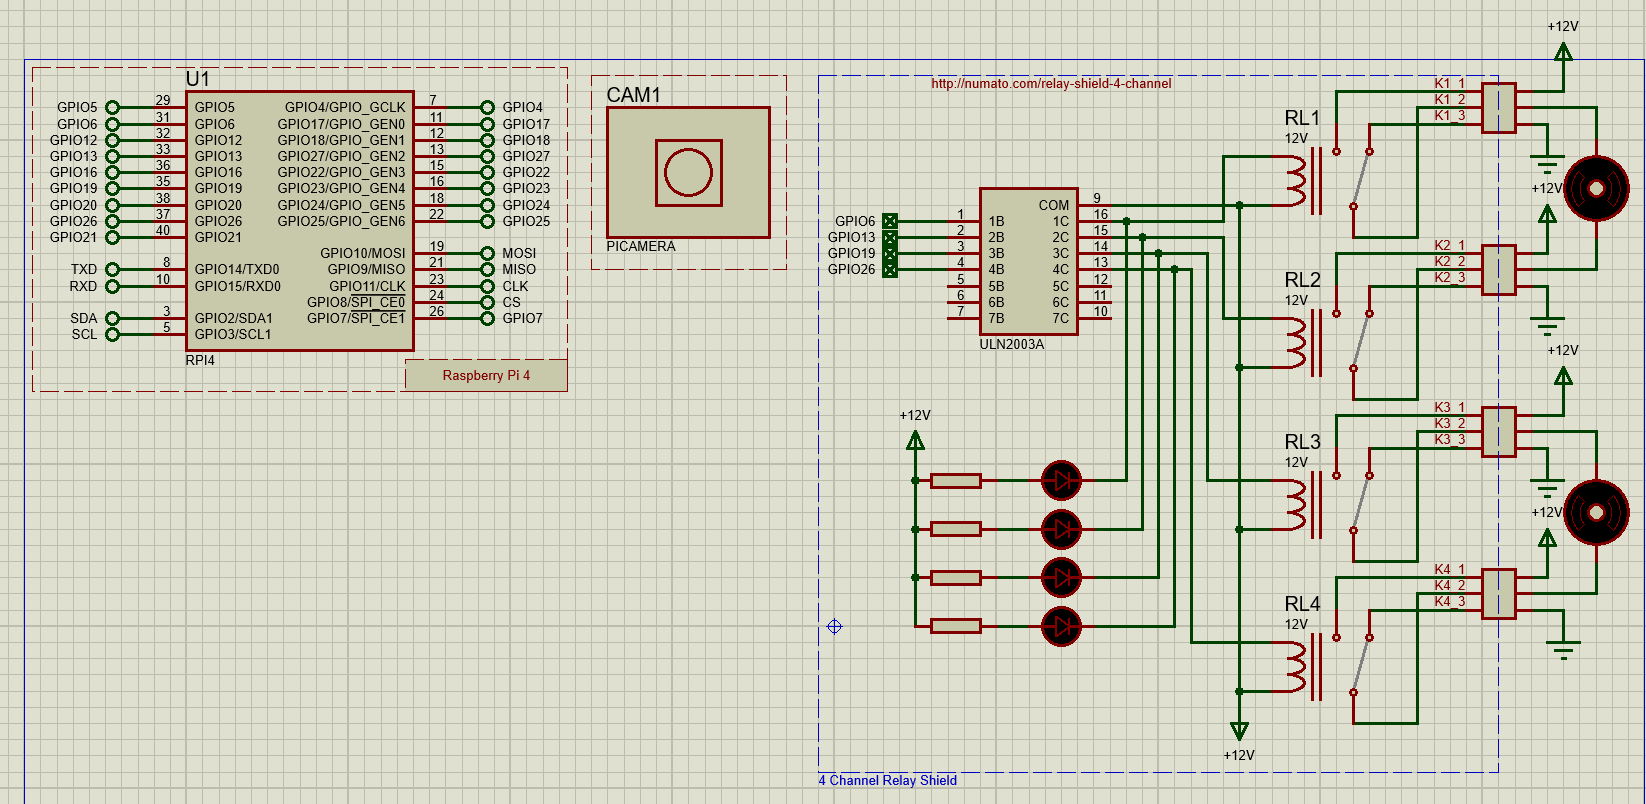
\includegraphics[width=0.9\textwidth]{h_bridge_schematic}
	\caption{Hardware Schematic}
	\label{fig:h_bridge_fig}
\end{figure}

In figure \ref{fig:h_bridge_fig} presents the electronic circuit diagram,
designed using Proteus. The diagram illustrates a system where a Raspberry Pi 4
serves as the central control unit, managing four motors through a relay
mechanism. The Raspberry Pi 4, represented by a rectangular box on the left,
showcases various pin connections, including GPIO pins, power supply pins (5V
and 3V3), ground pins (GND), and communication pins (TXD, RXD, SDA, SCL).

In the center of the diagram, an 18-pin integrated circuit labeled "ULN2803A" is
depicted. This component, a Darlington transistor array, likely functions as a
buffer, providing the necessary current to drive the relays. Four relays,
designated as RL1, RL2, RL3, and RL4, are positioned on the right side of the
diagram, each connected to a motor (represented by a circle with an "M" inside)
and a +12V power source. Additionally, four resistors are placed between the
ULN2803A and the relays, serving to limit current. The circuit section
containing these resistors is labeled "4 Channel Relay Driver," indicating its
purpose.

The camera module is labeled "PICAMERA" is located in the top center of the
diagram. It is represented by a square with a circle inside, symbolizing the
camera lens. The camera module is connected to the Raspberry Pi 4 through the
CSI (Camera Serial Interface) pins. The overall circuit is designed for a 12V
system, with the +12V power supply indicated at various points. The Raspberry Pi
4's GPIO pins are used to control the relays.

\section{Hardware Considerations}
The hardware components include high-resolution cameras, lighting systems for consistent image capture, and 
microcontrollers like Raspberry Pi or Arduino for system control, actuators like DC and stepper motors to move 
the mangoes. The choice of hardware is justified based on cost, performance, and compatibility with the software framework.

\subsection{General Prototype Framework}
\begin{figure}[!htbp]
	\centering
	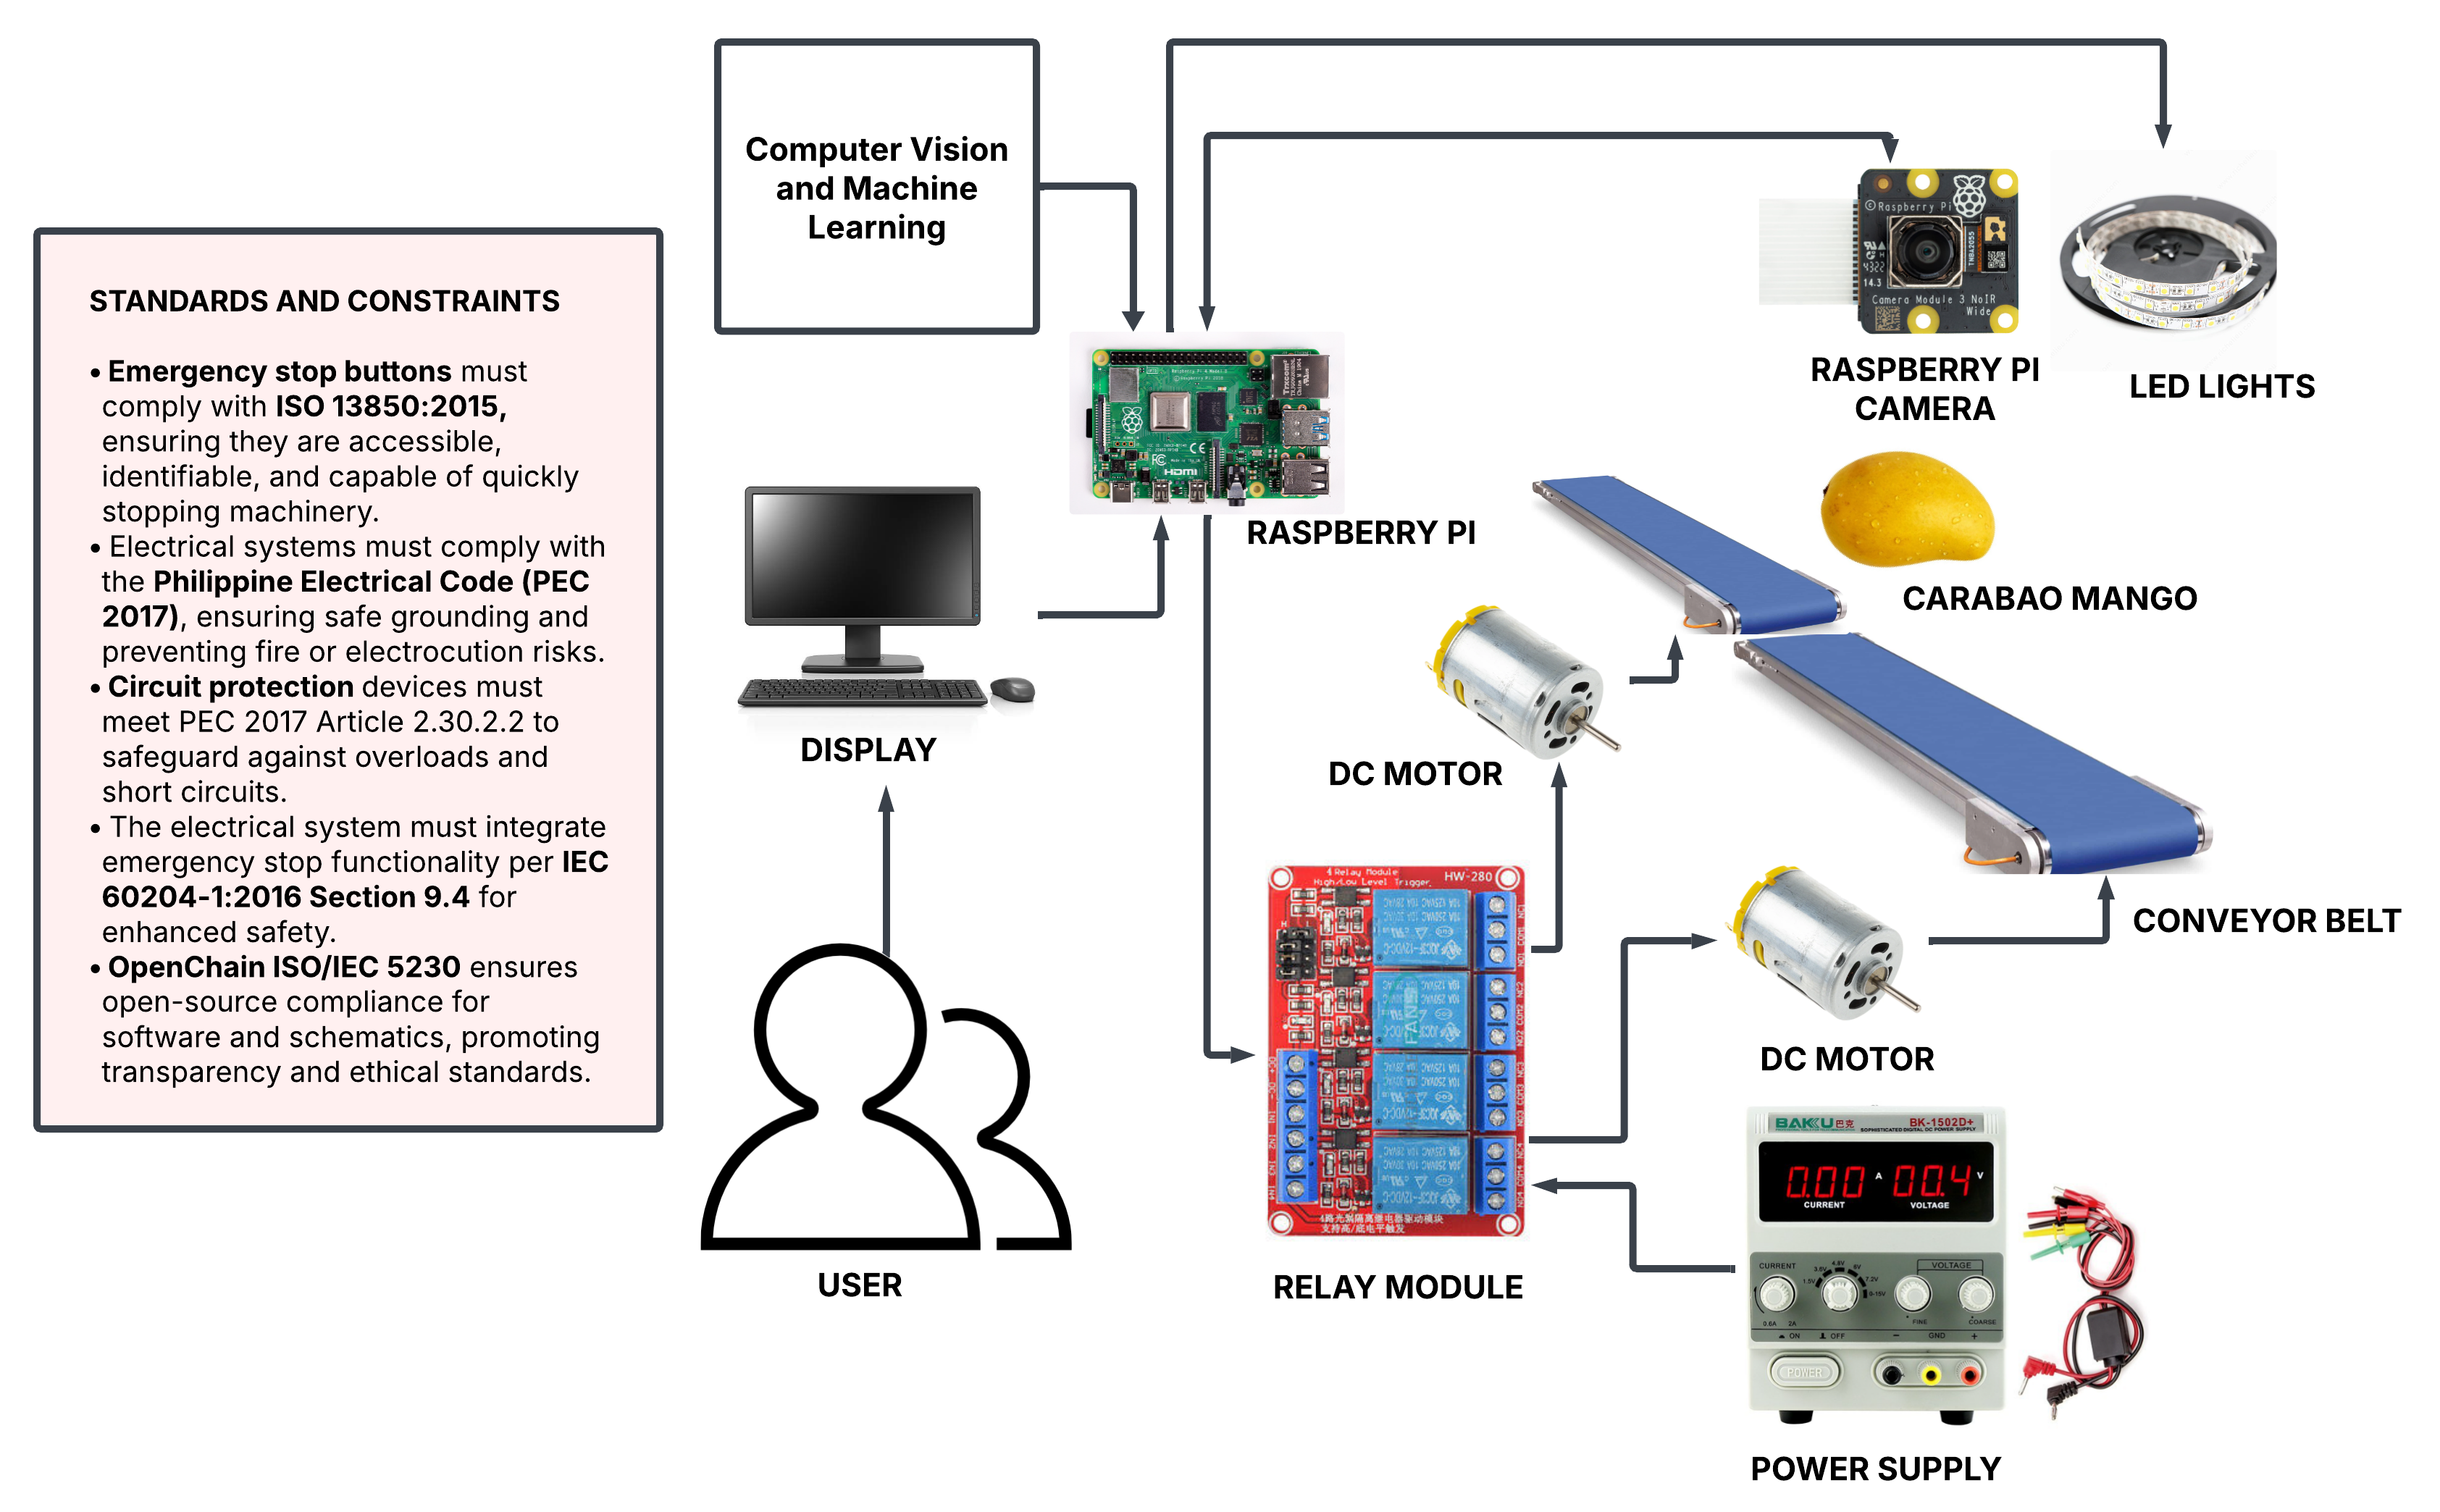
\includegraphics[width=0.9\textwidth]{pro2typediagram}
	\caption{Prototype Framework}
	\label{fig:prototypeDiagram_fig}
\end{figure}

\subsection{Prototype Flowchart}
\begin{figure}[!htbp]
	\centering
	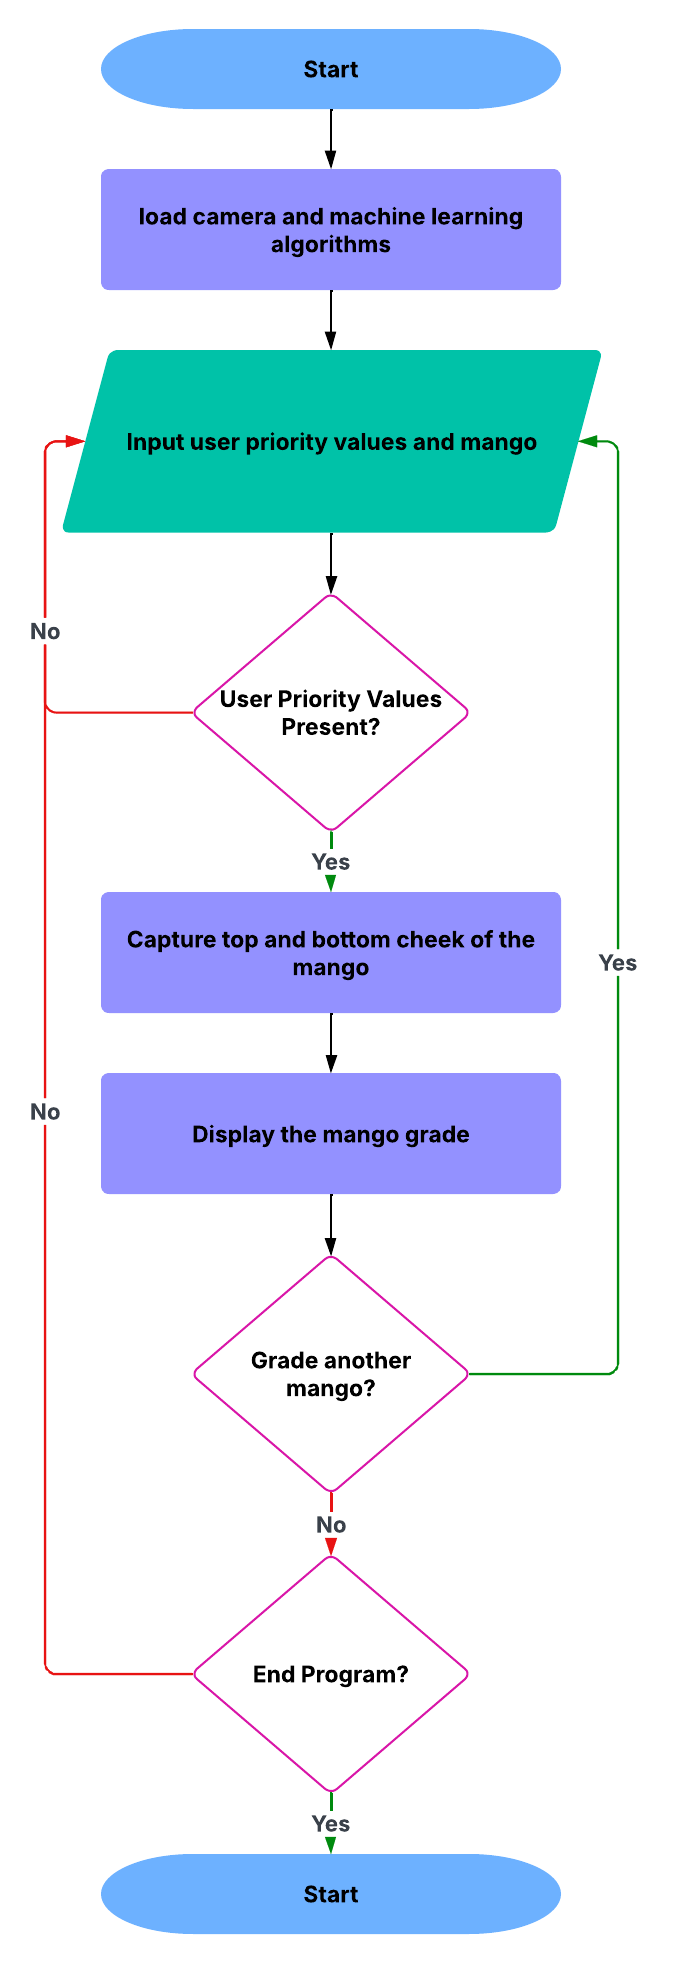
\includegraphics[width=0.40\textwidth]{mainFlowchart}
	\caption{Prototype Main Flowchart}
	\label{fig:pro2typeDiagram_fig}
\end{figure}

\subsection{Prototype 3D Model}
\begin{figure}[!htbp]
	\centering
	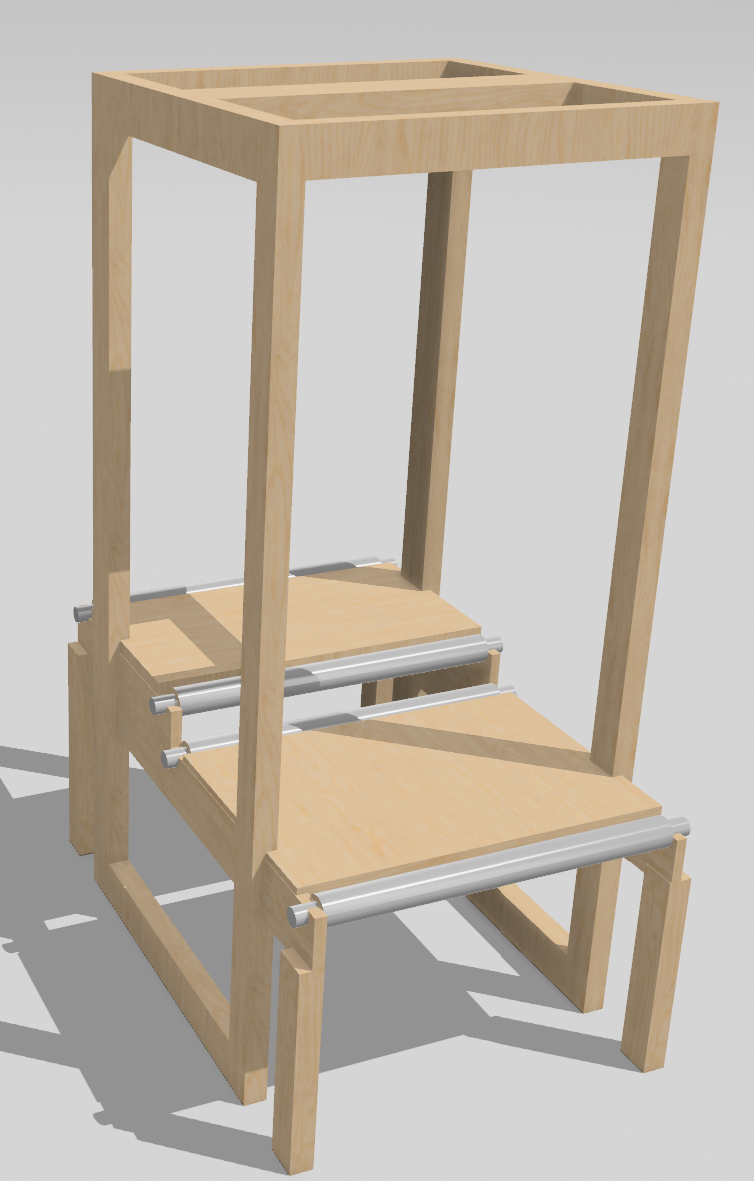
\includegraphics[width=0.60\textwidth]{3D_Drawing}
	\caption{Initial 3D Model of the Prototype}
	\label{fig:3dModel_fig}
\end{figure}


\subsection{Hardware Specifications}

\subsubsection{Raspberry Pi}
\begin{figure}[!htbp]
	\centering
	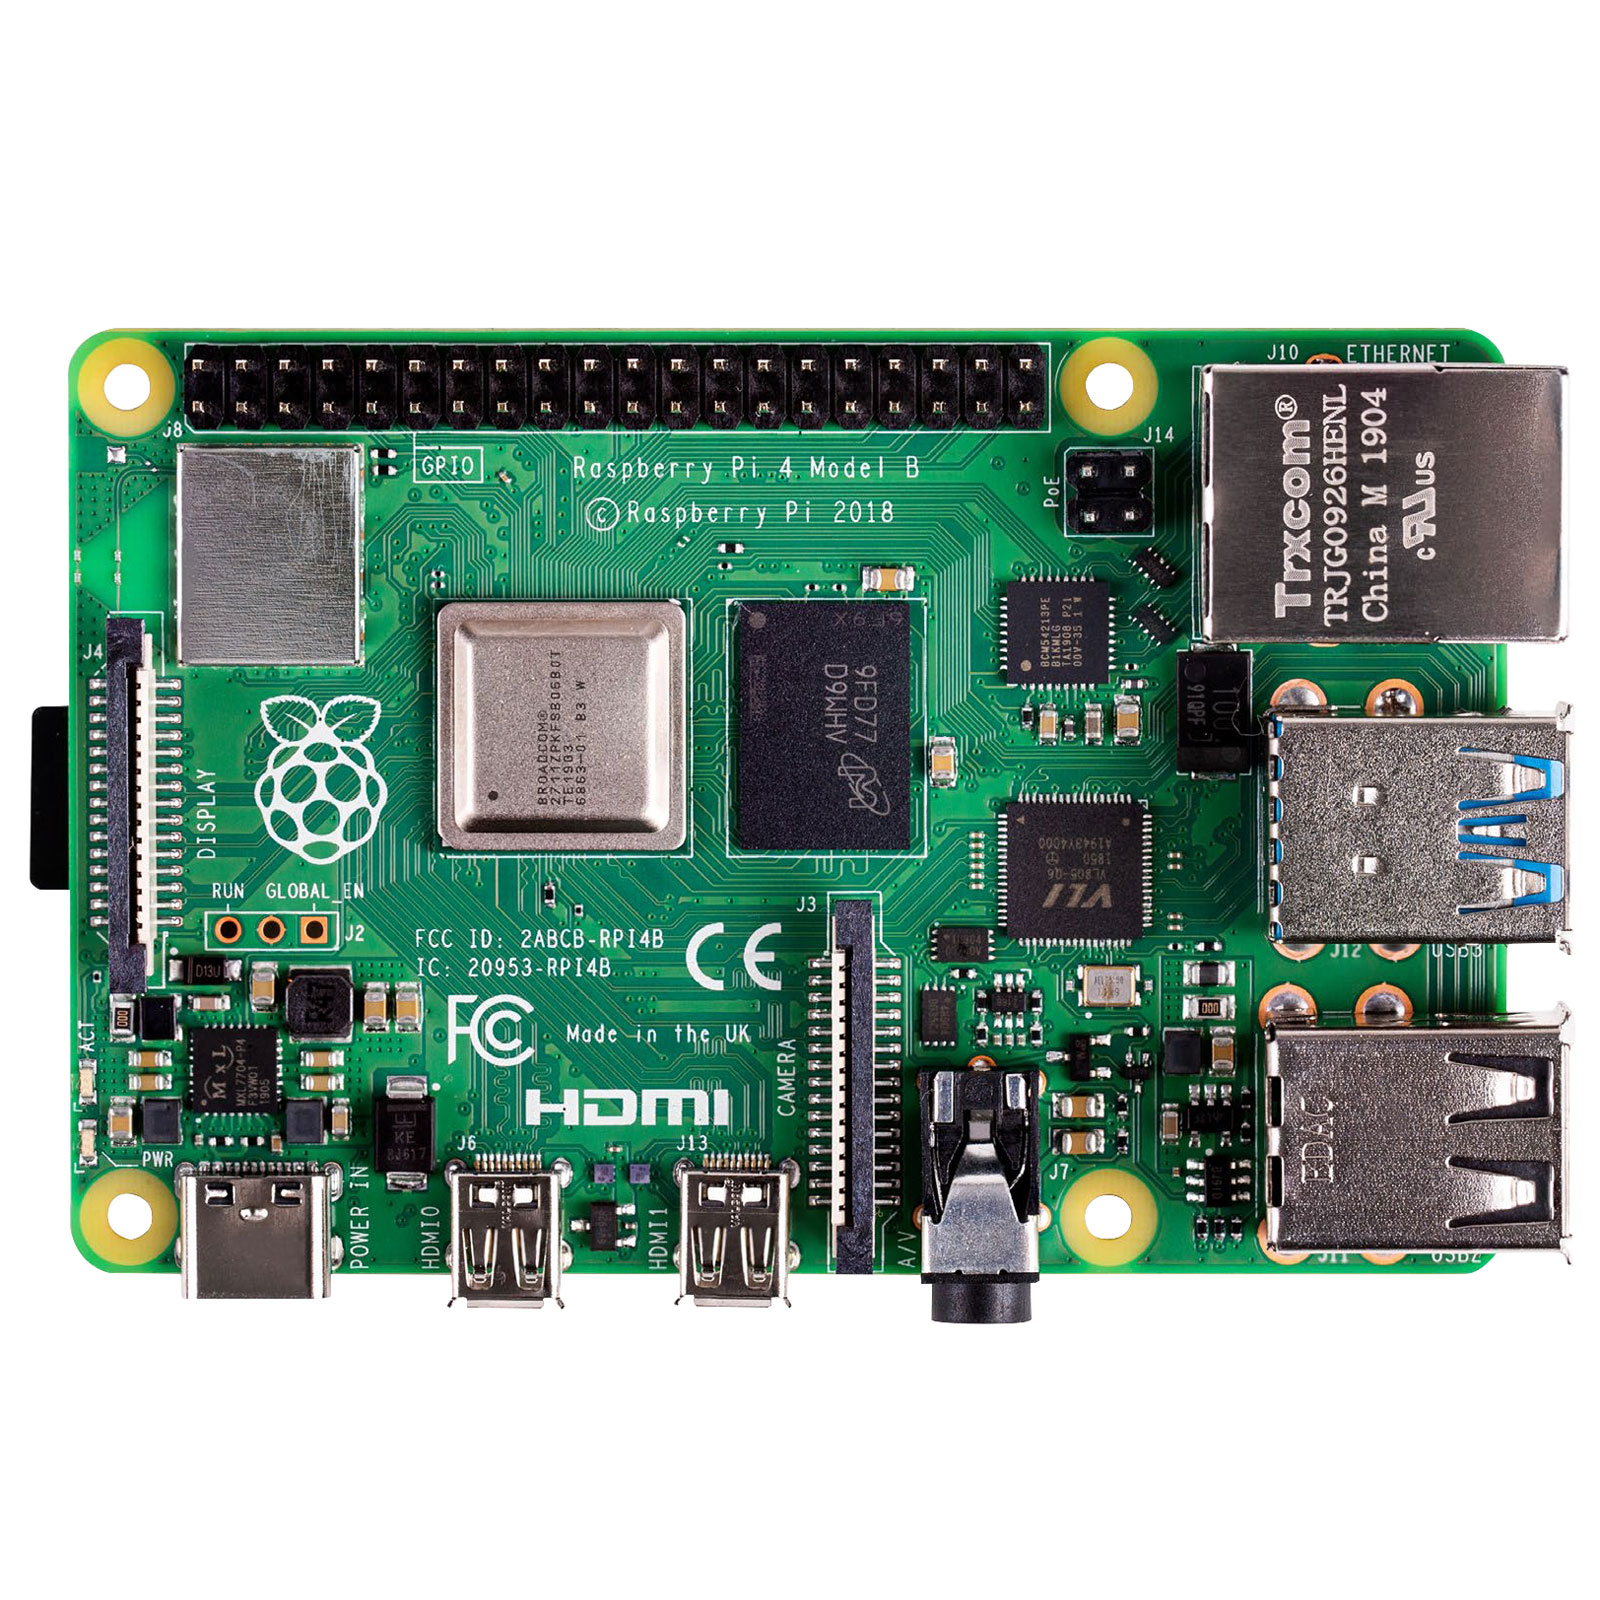
\includegraphics[width=0.5\textwidth]{rpi4b}
	\caption{Raspberry Pi 4 Model B}
	\label{fig:rpi4b_fig}
\end{figure}
The Raspberry Pi 4 Model B is a compact, low-cost computer that serves as the system's main processing unit. 
It was chosen for its balance of performance and affordability, making it suitable for image processing tasks.
Furthermore, it was selected for its compatibility with various peripherals through the GPIO pins and USB-A ports together
with its ease of integration into the prototype.
\\
\\
\textbf{Specifications:}
\begin{itemize}
    \item SoC: Broadcom BCM2711
    \item CPU: Quad-core ARM Cortex-A72 (64-bit)
    \item Clock Speed: 1.5 GHz (base, overclockable)
    \item RAM: 8GB LPDDR4-3200 SDRAM
    \item Wireless: Dual-band 2.4 GHz / 5 GHz Wi-Fi (802.11ac)
    \item Bluetooth: Bluetooth 5.0 (BLE support)
    \item Ethernet: Gigabit Ethernet (full throughput)
    \item USB: 2 x USB 3.0 ports and 2 x USB 2.0 ports
    \item Video Output: 2 x micro-HDMI ports (supports 4K @ 60Hz, dual 4K display capability)
    \item Audio: 3.5mm audio/video composite jack
    \item Storage: MicroSD card slot (supports booting via SD card or USB)
    \item GPIO: 40-pin GPIO header (backward-compatible with older models)
    \item Camera/Display: CSI (camera) and DSI (display) ports
    \item Power Input: USB-C (5V/3A recommended)
    \item Power Consumption: ~3W idle, up to 7.5W under load
\end{itemize}

\subsubsection{Raspberry Pi Camera}
\begin{figure}[!htbp]
	\centering
	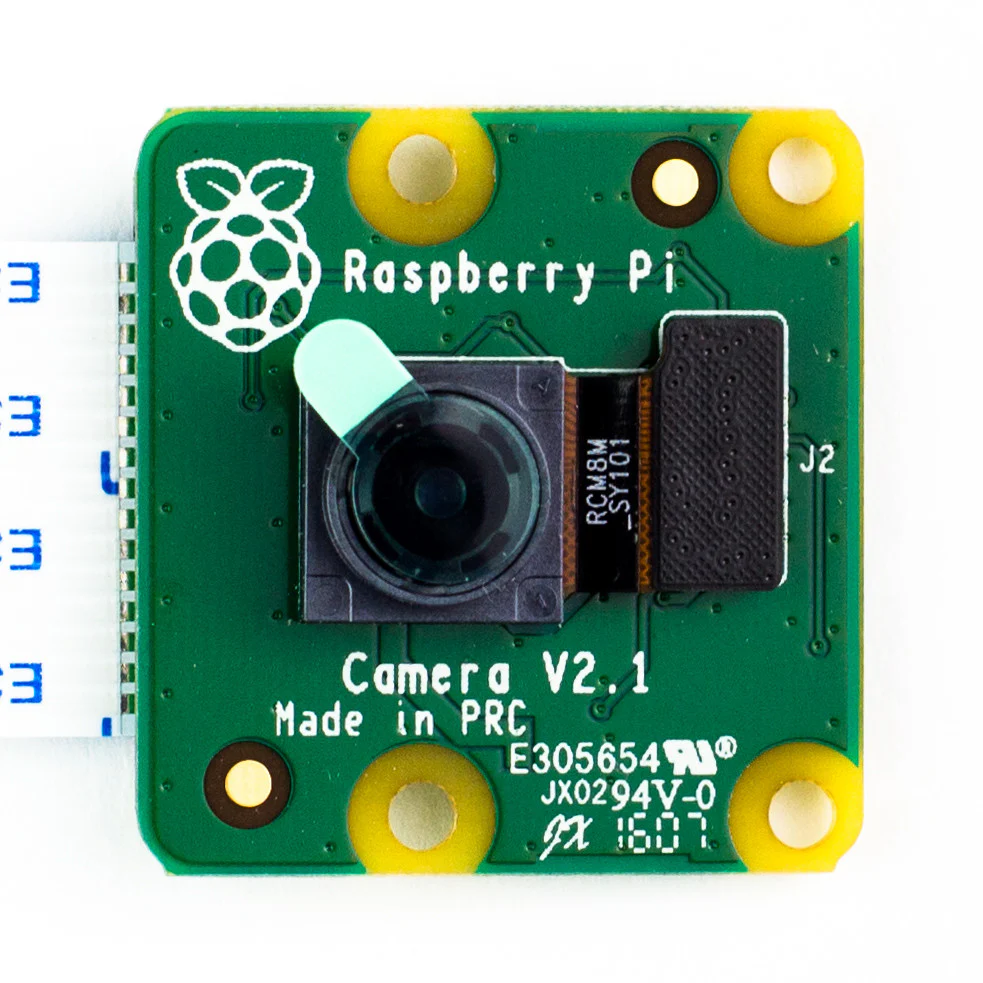
\includegraphics[width=0.5\textwidth]{rpi_cam}
	\caption{Raspberry Pi Camera Module Version 2}
	\label{fig:rpi_cam_fig}
\end{figure}
The Raspberry Pi Camera Module Version 2 is a high-quality camera module designed for the Raspberry Pi platform.
Likewise, it is capable of capturing still images at 8 megapixels, and supports video recording at 1080p @ 30fps, 
720p @ 60fps, and 480p @ 90fps. 
Moreover, it has a fixed-focus lens with a diagonal field of view of 62.2 degrees, and an optical format of 1/4 inch. 
Furthermore, it supports various Python libraries such as Picamera and OpenCV for image capture and processing.
As such, it was selected for its compact size, ease of integration, and ability to capture high-resolution images. 
\\
\\
\textbf{Specifications:}
\begin{itemize}
    \item Sensor: Sony IMX219PQ 8-megapixel CMOS sensor.
    \item Still Images Resolution: 8 MP (3280 x 2464 pixels).
    \item Video Resolution: Supports up to 1080p @ 30fps, 720p @ 60fps, and 480p @ 90fps.
    \item Focus: Fixed-focus lens (manual focus adjustment not supported without physical modification).
    \item Lens Size: 1/4-inch optical format.
    \item Field of View (FoV): Diagonal 62.2 degrees.
    \item Interface: Connected via 15-pin ribbon cable to the Raspberry Pi's CSI (Camera Serial Interface) port.
    \item APIs/Libraries: Supports Python libraries such as Picamera and OpenCV for image capture and processing.
    \item Dimensions: 25 mm x 24 mm x 9 mm.
\end{itemize}

\subsubsection{DC Motor}
\begin{figure}[!htbp]
	\centering
	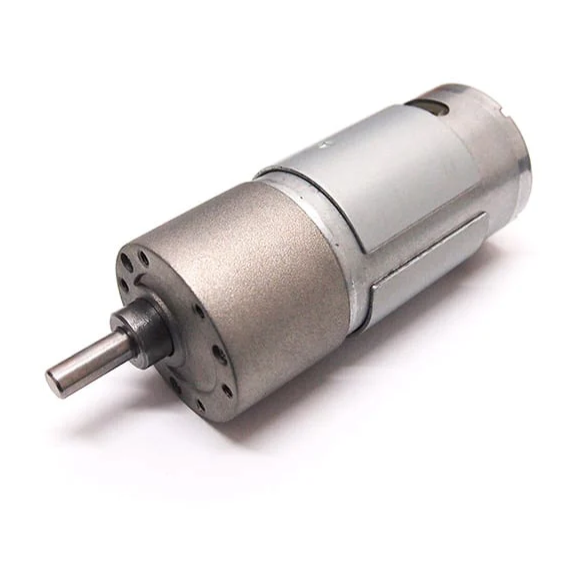
\includegraphics[width=0.5\textwidth]{dc_motor}
	\caption{12 Volt DC Gear Motor}
	\label{fig:dc_motor_fig}
\end{figure}
The 12 Volt DC Gear Motor is a compact, high-torque, and low-noise motor suitable for a 
wide range of applications, including robotics, automation, and industrial control systems. 
It features a spur gear design, which provides a high reduction ratio for increased torque output. 
The motor is designed for continuous operation and has a low power consumption under standard load 
conditions. Likewise, it is also capable of withstanding high temperatures and has a high reliability.
This motor was selected for its high torque output, low power consumption, and compact size, 
making it ideal for the conveyor system.
\\
\\
\textbf{Specifications:}
\begin{itemize}
    \item Gearbox Type: Spur gear design
    \item Operating Voltage: 12V (operational range: 6-12V)
    \item No-load Current Consumption: 0.8A
    \item Rated Current Draw: 3A (under standard load)
    \item No-load Speed: 282 RPM (maximum)
    \item Operating Speed: 248 RPM (under rated load)
    \item Torque Output: 18 kg-cm (rated)
    \item Stall Torque: 60 kg-cm (maximum)
    \item Power Rating: 50W (maximum)
    \item Unit Weight: 350 grams
\end{itemize}


\subsubsection{MicroSD Card}
\begin{figure}[!htbp]
	\centering
	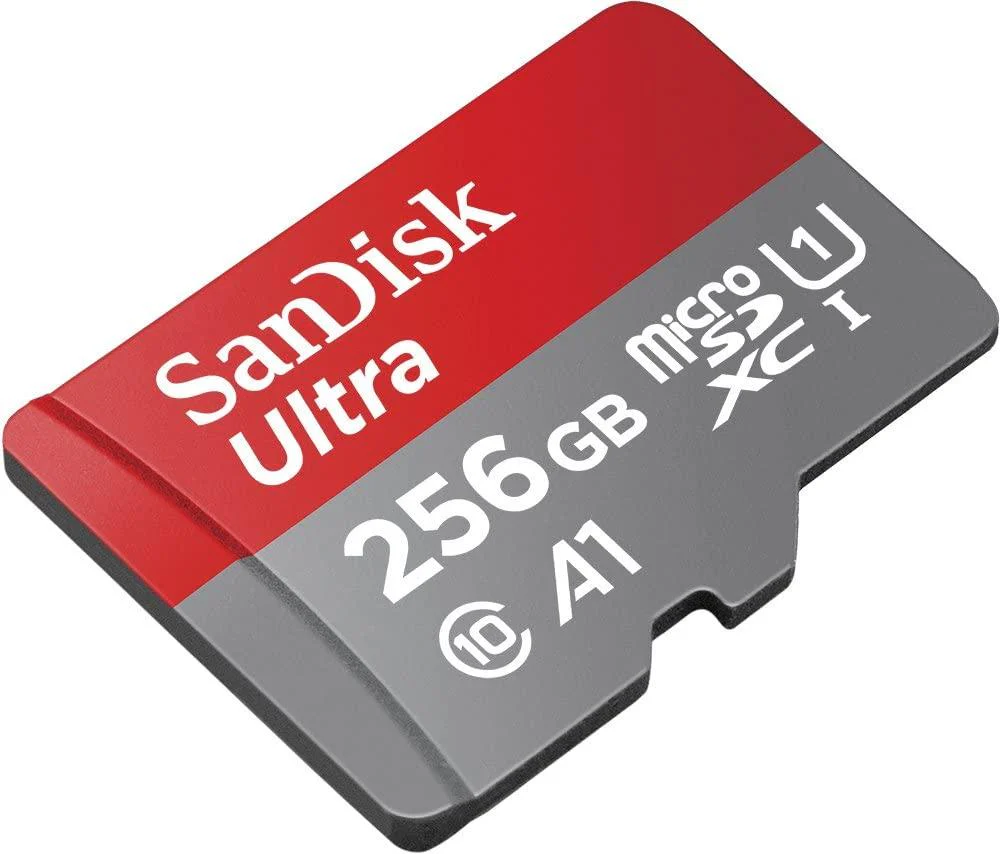
\includegraphics[width=0.5\textwidth]{sdCard}
	\caption{SanDisk Ultra MicroSD Card}
	\label{fig:sdCard_fig}
\end{figure}
The SanDisk Ultra MicroSD Card is a compact, high-capacity, and secure digital memory card 
that is suitable for a wide range of applications, including digital cameras, smartphones, and tablets.
It features a high-speed data transfer rate, making it ideal for storing large files such as images and videos.
This card was selected for its high capacity, secure data protection, and ease of use,
making it ideal for the storage system for the prototype. 
\\
\\
\textbf{Specifications:}
\begin{itemize}
    \item Capacity: 256GB
    \item Type: MicroSDXC (Secure Digital eXtended Capacity)
    \item Form Factor: MicroSD (11mm x 15mm x 1mm)
    \item File System: Pre-formatted exFAT
\end{itemize}

\subsubsection{LED Lights}
\begin{figure}[!htbp]
	\centering
	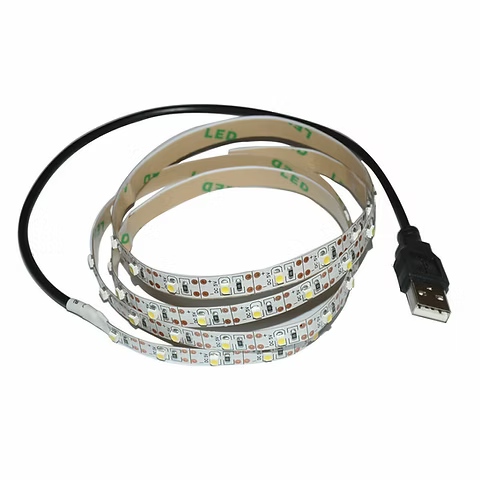
\includegraphics[width=0.5\textwidth]{led}
	\caption{LED Light Strip}
	\label{fig:led_fig}
\end{figure}
For the \gls{LED}, they were used to provide consistent lighting for image capture, ensuring accurate color representation and feature extraction.
The LED lights were selected for their energy efficiency, long lifespan, and ability to produce a uniform light output.
\\
\\
\textbf{Specifications:}
\begin{itemize}
    \item Power Input: 5V DC (USB-powered, compatible with laptops, power banks, or USB adapters).
    \item Waterproof Design: Suitable for indoor/outdoor use.
    \item LED Type: SMD 2835 (surface-mount diodes for high brightness and efficiency).
    \item Color Type: White (cool white)
    \item Length: 1m 
    \item Beam Angle: 120°
    \item Operating Temperature: -25°C to 60°C.
    \item Storage Temperature: -40°C to 80°C.
\end{itemize}


\subsubsection{Power Supply}
\begin{figure}[!htbp]
	\centering
	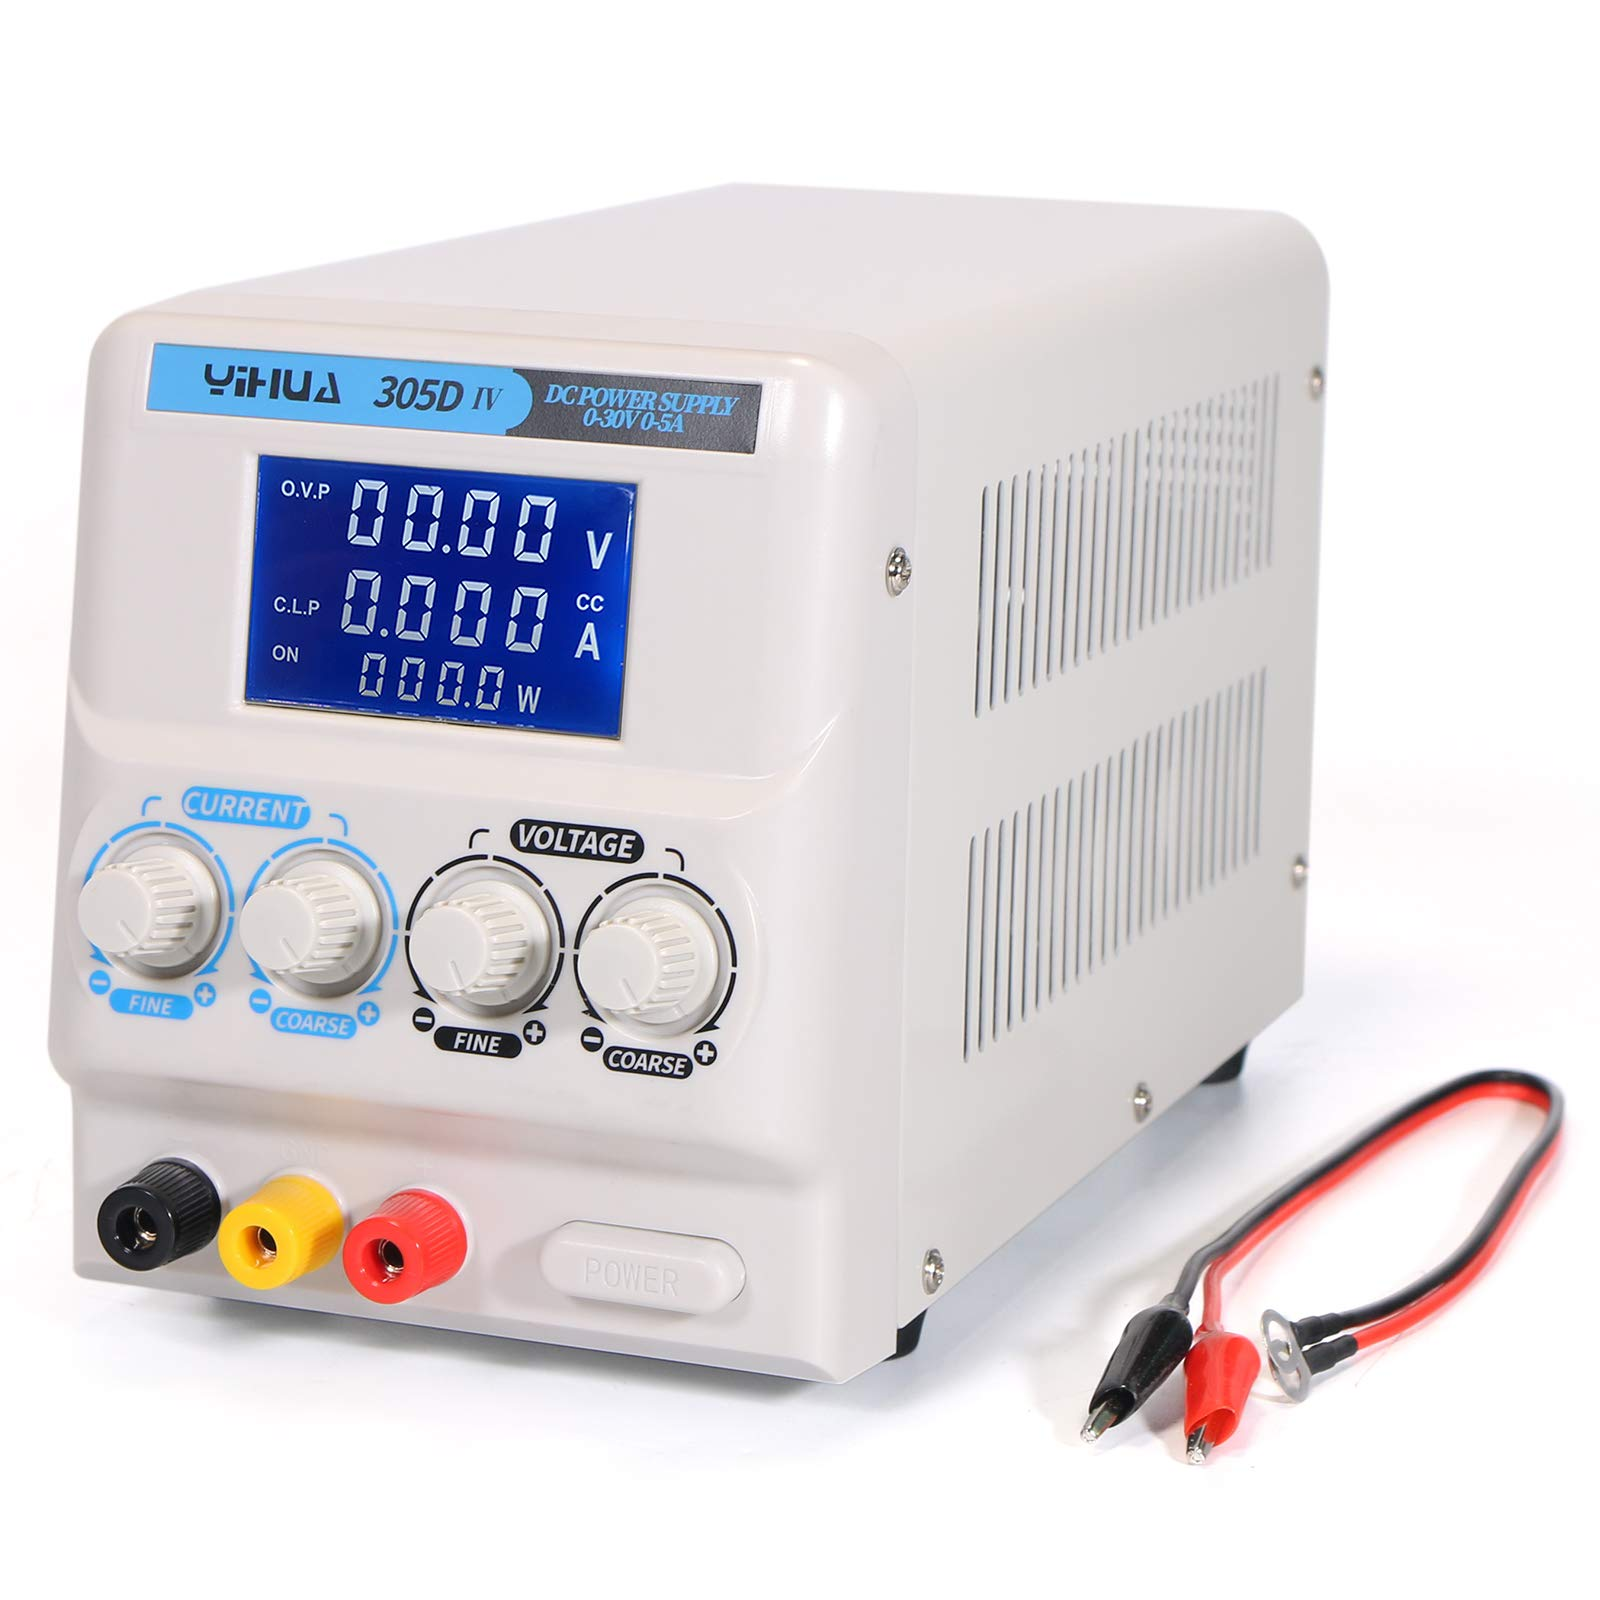
\includegraphics[width=0.5\textwidth]{Power_Supply}
	\caption{Bench Power Supply}
	\label{fig:Power_Supply_fig}
\end{figure}
The bench power supply is a versatile and adjustable power source used to 
provide stable voltage and current for various electronic projects.
It is designed for testing applications, allowing users to set specific voltage and current levels.
This power supply was selected for its versatility, 
ease of use, and ability to provide accurate voltage and current control for the prototype.
\\
\\
\textbf{Specifications:}
\begin{itemize}
    \item Type: SMPS (Switch-Mode Power Supply)
    \item Input: 110V AC, 50/60Hz (U.S. Standard)
    \item Output Range: 0-30V DC / 0-5A DC
    \item Voltage Precision: ±0.010V (10 mV) resolution
    \item Current Precision: ±0.001A (1 mA) resolution
    \item Power Precision: ±0.1W resolution
    \item Weight: 5 lbs (2.27 kg)
    \item Dimensions: 11.1" x 4.92" x 6.14" (28.2 cm x 12.5 cm x 15.6 cm)
    \item Maximum Power: 195W
    \item Power Source: AC input only
\end{itemize}

\subsubsection{4 Channel Relay Module}
\begin{figure}[!htbp]
	\centering
	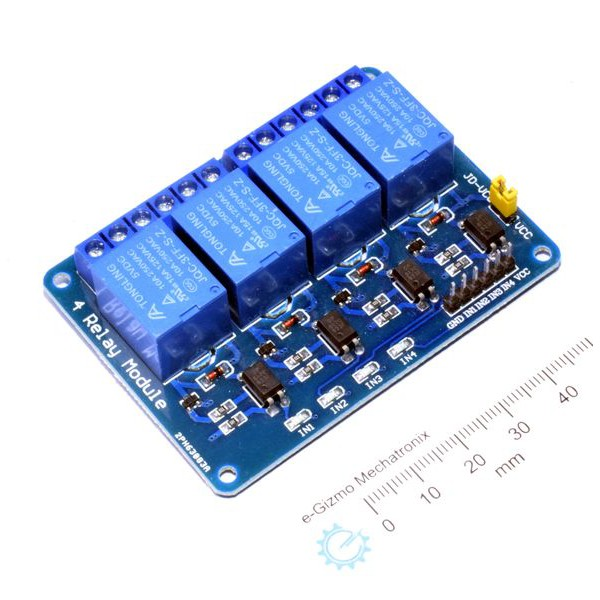
\includegraphics[width=0.5\textwidth]{relay_module}
	\caption{4 Channel Relay Module}
	\label{fig:relay_module_fig}
\end{figure}
The 4 Channel Relay Module is a compact and versatile relay 
board that allows for the control of multiple devices using a single microcontroller.
This module was selected for its compact size, ease of use, and ability to control multiple devices simultaneously.
It is designed to be used with microcontrollers such as Arduino and Raspberry Pi,
allowing for easy integration into the prototype.
\\
\\
\textbf{Specifications:}
\begin{itemize}
    \item Operating Voltage: 5V DC (compatible with Arduino, Raspberry Pi, and other microcontrollers).
    \item Number of Relays: 4 independent channels.
    \item Relay Type: Electromechanical (mechanical switching).
    \item Max AC Load: 10A @ 250V AC (resistive).
    \item Max DC Load: 10A @ 30V DC (resistive).
    \item Contact Type: SPDT (Single Pole Double Throw) - NO (Normally Open), NC (Normally Closed), COM (Common).
    \item Dimensions: ~50mm x 70mm x 20mm 
    \item Weight: ~50-80 grams.
    \item Status LEDs: Individual LEDs for each relay (indicates ON/OFF state).
    \item Input Pins: 4 digital control pins (one per relay).
    \item Output Terminals: Screw terminals for connecting loads (NO/NC/COM).
\end{itemize}

\section{Software Considerations}
The software stack includes Python for programming PyTorch for machine learning and OpenCV for image processing. These tools are selected for their robustness, ease of use, and extensive community support, ensuring efficient system development.

\subsection{PyTorch}

\subsection{OpenCV}

\subsection{Tkinter}

\subsection{CustomTkinter}

\section{Security and Reliability Considerations}
Potential vulnerabilities, such as data corruption during image capture, are addressed through redundancy and error-checking mechanisms. Reliability is ensured by implementing fault-tolerant designs and rigorous testing protocols.

\section{Scalability and Efficiency Considerations}
The system is designed to handle large volumes of mangoes by optimizing the machine learning model and using parallel processing techniques. Efficiency is improved through techniques like model quantization and hardware acceleration.

\section{User Interface}
A \gls{UI} is designed to display grading results, system status. Wireframes illustrate the layout, ensuring usability and accessibility for operators. 
Likewise, a \gls{GUI} is also used to allow users to customize the system's grading priorities.

\section{Constraints and Limitations}
Challenges include variations in mango appearance due to lighting and environmental factors. Trade-offs are made between model complexity and real-time performance to balance accuracy and speed.

\section{Technical Standards}
The system adheres to industry standards for image processing and machine learning, ensuring compatibility and interoperability with other systems.

\section{Prototyping and Simulation}
Prototypes are developed using tools like MATLAB and Simulink to simulate the system’s performance. These simulations help identify design flaws and optimize the system before deployment.,

\section{Design Validation}
The design is validated through testing, including unit testing of individual modules and integration testing of the entire system. Peer reviews and iterative improvements ensure the system meets the desired performance metrics.

\section{Summary}
This chapter outlined the key design considerations, including system architecture, hardware and software choices, and validation methods. These decisions are critical for developing a reliable and efficient mango sorting and grading system.

